\scanpage{31}
\margin{\figure{\begin{tikzpicture}[x=1cm,y=1cm]\draw (.12,.32)--(.1,.08)..controls(.09,.01)and(.02,.01)..(0,.05);\end{tikzpicture}}}
\margin{\figure{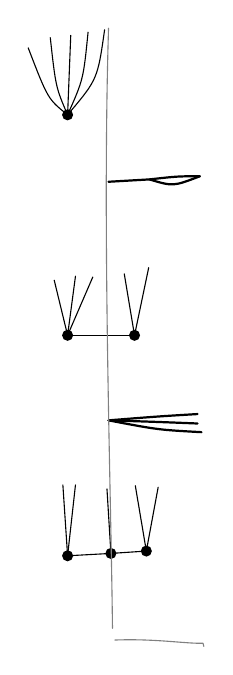
\begin{tikzpicture}[x=1cm,y=1cm,line cap=round,line join=round]
\fill (0,6.2) circle(2pt);
\draw (0,6.2)..controls(-.25,6.4)..(-.5,7.05);
\draw (0,6.2)..controls(-.15,6.55)..(-.22,7.18);
\draw (0,6.2)--(.04,7.21);
\draw (0,6.2)..controls(.2,6.65)..(.26,7.25);
\draw (0,6.2)..controls(.38,6.65)..(.47,7.28);
\draw (0,3.4)--(.85,3.4);\fill (0,3.4) circle(2pt);\fill (.85,3.4) circle(2pt);
\draw (0,3.4)--(-.17,4.1);\draw (0,3.4)--(.1,4.15);\draw (0,3.4)--(.32,4.14);
\draw (.85,3.4)--(.72,4.18);\draw (.85,3.4)--(1.03,4.26);
\draw (0,.6)--(.55,.63)--(1,.66);
\foreach \x/\y in {0/.6,.55/.63,1/.66}{\fill (\x,\y) circle(2pt);}
\draw (0,.6)--(-.06,1.5);\draw (0,.6)--(.1,1.5);\draw (.55,.63)--(.5,1.45);\draw (1,.66)--(.86,1.49);\draw (1,.66)--(1.15,1.47);
% Literal courses of the two retraced marginal arrows.
\draw[thick] (.52,5.35)--(1.04,5.38)..controls(1.4,5.42)..(1.68,5.42);
\draw[thick] (1.68,5.42)..controls(1.34,5.29)..(1.04,5.38);
\draw[thick] (.52,2.32)..controls(1.15,2.37)..(1.65,2.4);
\draw[thick] (.52,2.32)..controls(1.15,2.3)..(1.65,2.28);
\draw[thick] (.52,2.32)..controls(1.15,2.2)..(1.7,2.17);
\draw[gray] (.52,7.3)..controls(.44,4.7)and(.55,1.5)..(.57,-.32);
\draw[gray] (.6,-.47)..controls(1.12,-.45)and(1.52,-.52)..(1.72,-.51)--(1.73,-.55);
\end{tikzpicture}}}


\diagram{\begin{tikzcd}[ampersand replacement=\&,column sep=9em,row sep=10em]
\begin{gathered}\mathrm{I}_{10}\ (\text{pentagonale})\\
\vcenter{\hbox{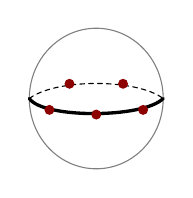
\begin{tikzpicture}[x=.85cm,y=.85cm,line cap=round,line join=round]
\draw[gray] (0,0) ellipse (1 and 1.05);
\draw[very thick] (-1,0)..controls(-.8,-.3)and(.7,-.3)..(1,0);
\draw[dash pattern=on 1.7pt off 1.5pt] (-1,0)..controls(-.6,.3)and(.6,.3)..(1,0);
\fill[red!55!black] (-.7,-.17) circle(1.8pt);
\fill[red!55!black] (0,-.24) circle(1.8pt);
\fill[red!55!black] (.7,-.17) circle(1.8pt);
\fill[red!55!black] (-.4,.22) circle(1.8pt);
\fill[red!55!black] (.4,.22) circle(1.8pt);
\end{tikzpicture}}}\\
\text{12 structures pentagonales sur }K\\
\{\sigma,\sigma^{-1}\}\in P_2(\mathrm{Circ}(K)\\
G\simeq\mathbb D_5\\
\widetilde G\simeq\mathbb D_5\times\{1,\sigma\}\end{gathered}\&\begin{gathered}\mathrm I_6\ (\text{bitétraédrale})\\
\vcenter{\hbox{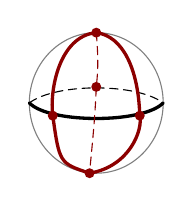
\begin{tikzpicture}[x=.85cm,y=.85cm,line cap=round,line join=round]
\draw[gray] (0,0) ellipse (1 and 1.05);
\draw[very thick] (-1,0)..controls(-.7,-.31)and(.7,-.31)..(1,0);
\draw[densely dashed] (-1,0)..controls(-.6,.3)and(.6,.3)..(1,0);
\draw[red!55!black,very thick] (0,1.05)..controls(-.55,1)and(-.7,.2)..(-.65,-.19)..controls(-.55,-.9)..(-.1,-1.05)..controls(.5,-.95)and(.7,-.4)..(.65,-.19)..controls(.63,.5)and(.4,1)..(0,1.05);
\draw[red!55!black,densely dashed] (0,1.05)..controls(.03,.7)and(.03,.5)..(0,.24)..controls(-.02,-.3)and(-.08,-.8)..(-.1,-1.05);
\fill[red!55!black] (0,1.05) circle(1.8pt);
\fill[red!55!black] (-.65,-.19) circle(1.8pt);
\fill[red!55!black] (.65,-.19) circle(1.8pt);
\fill[red!55!black] (0,.24) circle(1.8pt);
\fill[red!55!black] (-.1,-1.05) circle(1.8pt);
\end{tikzpicture}}}\\
\text{20 structures }K=J\amalg\omega\\
\text{avec }\omega\xrightarrow{\sim}\underline\omega(J)\\
G\simeq\unsure{\mathfrak S|G}_J\simeq\unsure{\mathfrak S|G}_3\\
\widetilde G\simeq\unsure{\mathfrak S|G}_3\times\{1,\sigma\}\end{gathered} \arrow[r,"{3\quad f_{B,s}\quad2}","{(B\in\unsure{\mathrm{Bit\acute et}|\mathrm{Bitet}}(K),\ s\in T(B)=J)}"'] \& \begin{gathered}\mathrm I_4\ (\text{pyramidale})\\
\vcenter{\hbox{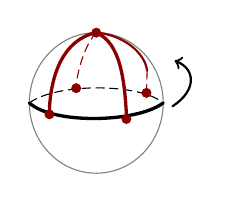
\begin{tikzpicture}[x=.85cm,y=.85cm,line cap=round,line join=round]
\draw[gray] (0,0) ellipse (1 and 1.05);
\draw[very thick] (-1,0)..controls(-.65,-.32)and(.6,-.3)..(1,0);
\draw[densely dashed] (-1,0)..controls(-.6,.3)and(.65,.3)..(1,0);
\draw[red!55!black,very thick] (0,1.05)..controls(-.5,.95)and(-.68,.4)..(-.7,-.10);
\draw[red!55!black,very thick] (0,1.05)..controls(.36,.9)and(.42,.35)..(.45,-.16);
\draw[red!55!black,densely dashed] (0,1.05)..controls(-.15,.9)and(-.29,.5)..(-.3,.22);
\draw[red!55!black,thick] (0,1.05)..controls(.4,1.02)and(.73,.75)..(.76,.48);
\draw[red!55!black,densely dashed] (.76,.48)--(.75,.15);
\draw[->,thick] (1.14,-.05)..controls(1.52,.2)and(1.47,.52)..(1.17,.63);
\fill[red!55!black] (0,1.05) circle(1.8pt);
\fill[red!55!black] (-.7,-.17) circle(1.8pt);
\fill[red!55!black] (.45,-.24) circle(1.8pt);
\fill[red!55!black] (-.3,.22) circle(1.8pt);
\fill[red!55!black] (.75,.15) circle(1.8pt);
\end{tikzpicture}}}\\
\text{30 structures carrés orientés}\\
K\simeq\{P\}\amalg I\\
I\ \text{structure carrée \uline{orientée}}\ (Q,\omega)=\vec Q\\
I=\coprod_{\alpha\in\delta}\alpha\qquad\delta=\text{ens. des diagonales }\alpha\\
\omega\in\delta\wedge\bigwedge_{\alpha\in\delta}\alpha\\
G=\widetilde G=\mathbb Z/4\mathbb Z\end{gathered} \arrow[dl,bend right=10,pos=.27,"{4\quad f_{\vec Q,\omega,a}\quad2}","{(Q=\overrightarrow{\mathrm{Carr}}(K),\ a\in\Lambda(Q))}"'] \\
\begin{gathered}\mathrm{II}_2\ (\text{carré-triangle droit})\\
\vcenter{\hbox{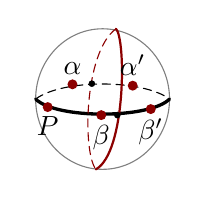
\begin{tikzpicture}[x=.85cm,y=.85cm,line cap=round,line join=round]
\draw[gray] (0,0) ellipse (1 and 1.05);
\draw[very thick] (-1,0)..controls(-.7,-.3)and(.7,-.3)..(1,0);
\draw[densely dashed] (-1,0)..controls(-.6,.3)and(.6,.3)..(1,0);
\draw[red!55!black,thick] (.2,1.05)..controls(.35,.9)and(.35,-.8)..(-.1,-1.05);
\draw[red!55!black,densely dashed] (.2,1.05)..controls(-.28,.7)and(-.3,-.8)..(-.1,-1.05);
\fill[red!55!black] (-.45,.22) circle(1.8pt) node[above,black] {$\alpha$};
\fill[red!55!black] (.45,.2) circle(1.8pt) node[above,black] {$\alpha'$};
\fill[red!55!black] (-.82,-.12) circle(1.8pt) node[below,black] {$P$};
\fill[red!55!black] (-.02,-.24) circle(1.8pt) node[below,black] {$\beta$};
\fill[red!55!black] (.72,-.15) circle(1.8pt) node[below,black] {$\beta'$};
\fill (-.16,.23) circle(1.2pt);\fill (.22,-.24) circle(1.2pt);
\end{tikzpicture}}}\\
\text{2 sommets-repères}\quad\deleted{\text{\unsure{repères}}}\\
\text{60 structures ``pentagone}\\
\text{avec sommet'' sur }K\\
\text{i.e. }K\simeq B\amalg\omega,\ \text{avec }\omega\hookrightarrow J\\
\text{i.e. }P\in J\text{ et }\omega\simeq\omega'=B\setminus\{P\}\\
G\simeq\mathbb Z/2\mathbb Z\\
\widetilde G\simeq\mathbb Z/2\mathbb Z\times\{1,\sigma\}\end{gathered} \arrow[u,"{1\quad\gamma_{\pi,s}\quad5}","{(\pi\in\mathrm{Pent}(K),\ s\in K)}"'] \arrow[r,"{1\quad\tau_{\pi,s}=\mathrm{tw}_{1/4}\quad1}"] \& \begin{gathered}\mathrm{II}'_2=\mathrm{Tw}_{1/4}\mathrm{II}_2\\
(\text{carré-triangle gauche})\\
\text{4 sommets}\ \deleted{\text{\unsure{repères}}}\\
\vcenter{\hbox{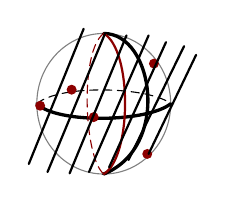
\begin{tikzpicture}[x=.85cm,y=.85cm,line cap=round,line join=round]
% The drawing is canceled by its seven oblique strokes. No alphabetic labels are secure beneath them.
\draw[gray] (0,0) ellipse (1 and 1.05);
\draw[very thick] (0,1.05)..controls(.75,1.05)and(1,-.65)..(0,-1.05);
\draw[very thick] (-1,0)..controls(-.7,-.3)and(.65,-.28)..(1,0);
\draw[densely dashed] (-1,0)..controls(-.65,.3)and(.7,.25)..(1,0);
\draw[red!55!black,thick] (0,1.05)..controls(.43,.8)and(.42,-.8)..(0,-1.05);
\draw[red!55!black,densely dashed] (0,1.05)..controls(-.36,.8)and(-.3,-.8)..(0,-1.05);
\fill[red!55!black] (-.95,-.03) circle(1.8pt);
\fill[red!55!black] (-.48,.21) circle(1.8pt);
\fill[red!55!black] (-.15,-.2) circle(1.8pt);
\fill[red!55!black] (.75,.6) circle(1.8pt);
\fill[red!55!black] (.65,-.75) circle(1.8pt);
\draw[thick] (-1.12,-.9)--(-.3,1.12);
\draw[thick] (-.84,-1.02)--(.02,1.05);
\draw[thick] (-.51,-1.04)--(.34,1.02);
\draw[thick] (-.22,-1.02)--(.67,1.02);
\draw[thick] (.08,-.95)--(.93,.92);
\draw[thick] (.37,-.84)--(1.2,.86);
\draw[thick] (.67,-.75)--(1.38,.73);
\end{tikzpicture}}}\quad\vcenter{\hbox{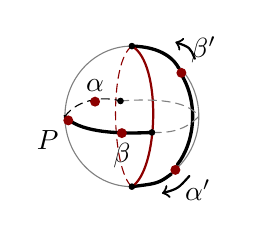
\begin{tikzpicture}[x=.85cm,y=.85cm,line cap=round,line join=round]
\draw[gray] (0,0) ellipse (1 and 1.05);
\draw[very thick] (0,1.05)..controls(.46,1.04)and(.64,.84)..(.7,.72);
\draw[very thick] (.76,.59)..controls(1,.16)and(.93,-.4)..(.68,-.72);
\draw[very thick] (.59,-.86)..controls(.4,-1)..(0,-1.05);
\draw[red!55!black,thick] (0,1.05)..controls(.45,.8)and(.4,-.8)..(0,-1.05);
\draw[red!55!black,densely dashed] (0,1.05)..controls(-.35,.8)and(-.3,-.8)..(0,-1.05);
\draw[very thick] (-1,0)..controls(-.8,-.22)and(-.3,-.27)..(.3,-.24);
\draw[densely dashed] (-1,0)..controls(-.8,.27)and(-.4,.3)..(-.17,.23);
\draw[gray,densely dashed] (-.17,.23)..controls(.48,.28)and(.86,.2)..(1,0)..controls(.8,-.2)and(.6,-.25)..(.3,-.24);
\fill[red!55!black] (-.55,.22) circle(1.8pt) node[above,black] {$\alpha$};
\fill[red!55!black] (.74,.65) circle(1.8pt) node[above right,black] {$\beta'$};
\fill[red!55!black] (-.95,-.06) circle(1.8pt) node[below left,black] {$P$};
\fill[red!55!black] (-.15,-.25) circle(1.8pt) node[below,black] {$\beta$};
\fill[red!55!black] (.65,-.8) circle(1.8pt) node[below right,black] {$\alpha'$};
\fill (0,1.05) circle(1.2pt);\fill (0,-1.05) circle(1.2pt);\fill (-.17,.23) circle(1.2pt);\fill (.3,-.24) circle(1.2pt);
\draw[->,thick] (.94,.86)..controls(.87,1.03)..(.65,1.11);
\draw[->,thick] (.86,-.89)..controls(.69,-1.08)..(.45,-1.15);
\end{tikzpicture}}}\\
\text{même paramétrage que }\mathrm{II}_2\\
G\simeq\mathbb Z/2\mathbb Z,\ \widetilde G\simeq\mathbb Z/2\mathbb Z\times\{1,\sigma\}\end{gathered} \arrow[u,"{\gamma'_{\pi,s}\quad3}","{\text{comp. avec }\unsure{\vec Q|\vec G};\ (\pi\in\mathrm{Pent}(K),\ s\in K)}"'] \& \begin{gathered}\mathrm{II}_1\ (\text{tétraèdre-triangle})\\
\vcenter{\hbox{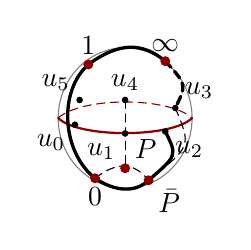
\begin{tikzpicture}[x=.85cm,y=.85cm,line cap=round,line join=round]
\draw[gray] (0,0) ellipse (1 and 1.05);
\draw[red!55!black,thick] (-1,0)..controls(-.7,-.3)and(.7,-.3)..(1,0);
\draw[red!55!black,densely dashed] (-1,0)..controls(-.65,.32)and(.65,.32)..(1,0);
\draw[very thick] (-.55,.8)..controls(-1,.4)and(-.95,-.5)..(-.45,-.9);
\draw[very thick] (-.55,.8)..controls(-.1,1.13)and(.25,1.14)..(.6,.85);
\draw[very thick,densely dashed] (.6,.85)..controls(.92,.5)..(.75,.15);
\draw[densely dashed] (.75,.15)..controls(.99,-.42)..(.35,-.93);
\draw[very thick] (.6,-.2)..controls(.78,-.56)..(.35,-.93);
\draw[very thick] (-.45,-.9)..controls(-.15,-1.1)and(.15,-1.12)..(.35,-.93);
\draw[densely dashed] (-.45,-.9)..controls(-.12,-.65)and(.12,-.65)..(.35,-.93);
\draw[densely dashed] (0,.27)--(0,-.75);
\fill[red!55!black] (-.55,.8) circle(1.8pt) node[above,black] {$1$};
\fill[red!55!black] (.6,.85) circle(1.8pt) node[above,black] {$\infty$};
\fill[red!55!black] (-.45,-.9) circle(1.8pt) node[below,black] {$0$};
\fill[red!55!black] (.35,-.93) circle(1.8pt) node[below right,black] {$\unsure{\bar P}$};
\fill[red!55!black] (0,-.75) circle(1.8pt) node[above right,black] {$\unsure{P}$};
\fill (-.75,-.1) circle(1.2pt) node[below left] {$u_0$};
\fill (0,-.23) circle(1.2pt) node[below left] {$u_1$};
\fill (.6,-.2) circle(1.2pt) node[below right] {$u_2$};
\fill (.75,.15) circle(1.2pt) node[above right] {$u_3$};
\fill (0,.27) circle(1.2pt) node[above] {$u_4$};
\fill (-.68,.27) circle(1.2pt) node[above left] {$u_5$};
\end{tikzpicture}}}\\
\text{6 sommets-repères}\\
\text{120 structures entièrement}\\
\text{épinglées,}\\
G=\deleted{\unsure{1}}=\{1\},\quad\widetilde G=\{1,\sigma\}\\
\left[\begin{gathered}K=J\amalg\varepsilon\quad\operatorname{card}J=3,\operatorname{card}\varepsilon=2\\\omega\in\underline\omega(J),\ r\in J\times\varepsilon\\\tau_r^0:\mathrm{II}_1(J,\varepsilon)\longrightarrow\mathrm{II}_1(u_\omega(r))\\\text{où }u_\omega=\omega\times(-1)\text{ sur }J\times\varepsilon\end{gathered}\right]\end{gathered} \arrow[ul,pos=.73,"{1\quad\gamma_r^0\quad6}","{\text{compat. avec }\unsure{\vec Q|\vec G}}"'] \arrow[loop right,"{\tau_r^0=\mathrm{tw}_{1/6}}"] \\
\begin{gathered}\mathrm{III}_2\ (\text{triple triangle droit})\\
\vcenter{\hbox{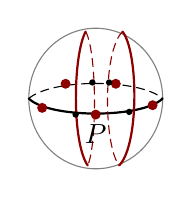
\begin{tikzpicture}[x=.85cm,y=.85cm,line cap=round,line join=round]
\draw[gray] (0,0) ellipse (1 and 1.05);
\draw[thick] (-1,0)..controls(-.7,-.3)and(.7,-.3)..(1,0);
\draw[densely dashed] (-1,0)..controls(-.65,.3)and(.65,.3)..(1,0);
\draw[red!55!black,thick] (-.15,1)..controls(-.34,.65)and(-.36,-.65)..(-.12,-1);
\draw[red!55!black,densely dashed] (-.15,1)..controls(.02,.7)and(.02,-.7)..(-.12,-1);
\draw[red!55!black,densely dashed] (.4,1)..controls(.1,.7)and(.12,-.7)..(.35,-1);
\draw[red!55!black,thick] (.4,1)..controls(.64,.7)and(.65,-.7)..(.35,-1);
\fill[red!55!black] (-.8,-.14) circle(1.8pt);
\fill[red!55!black] (0,-.24) circle(1.8pt);
\fill[red!55!black] (.85,-.1) circle(1.8pt);
\fill[red!55!black] (-.45,.22) circle(1.8pt);
\fill[red!55!black] (.3,.22) circle(1.8pt);\fill[black] (-.3,-.24) circle(1.15pt);
\fill[black] (.5,-.2) circle(1.15pt);
\fill[black] (-.05,.24) circle(1.15pt);
\fill[black] (.2,.24) circle(1.15pt);\node[below] at (0,-.25) {$P$};
\end{tikzpicture}}}\\
2+2\ \text{sommets-repère}\\
\text{60 structures ``pentagone avec}\\
\text{sommet'' sur }K,\\
G=\mathbb Z/2\mathbb Z,\widetilde G=\mathbb Z/2\mathbb Z\times\{1,\sigma\}\end{gathered} \arrow[u,start anchor=north west,"{2\quad\gamma_{\pi,\rho}\quad2}","{\begin{tikzpicture}[baseline]\draw (0,.15)..controls(-.12,.23)and(-.16,.3)..(-.14,.37);\end{tikzpicture}}"{pos=.02,description},"{(\pi\in\mathrm{Pent}(K),\rho\in\mathrm{Rep}\,\pi)}"'] \arrow[r,"{\unsure{\tau_{\pi,\omega}}}","{2\quad\tau_{\pi,\rho}=\mathrm{tw}_{1/4}\quad1}"'] \& \begin{gathered}\mathrm{III}_1\ (\text{triple triangle sem.-gauche})\\
\vcenter{\hbox{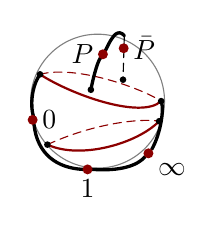
\begin{tikzpicture}[x=.85cm,y=.85cm,line cap=round,line join=round]
\draw[gray] (0,0) circle(1);
\draw[very thick] (-.86,.4)..controls(-1,.2)and(-1,-.1)..(-.96,-.22);
\draw[very thick] (-.95,-.35)..controls(-.9,-.8)and(-.6,-1)..(-.22,-1.02);
\draw[very thick] (-.08,-1.02)..controls(.35,-1.05)and(.6,-.96)..(.71,-.83);
\draw[very thick] (.81,-.72)..controls(.94,-.49)and(1,-.12)..(.95,0);
\draw[red!55!black,thick] (-.86,.4)..controls(-.4,.1)and(.65,-.28)..(.95,0);
\draw[red!55!black,densely dashed] (-.86,.4)..controls(-.35,.54)and(.6,.22)..(.95,0);
\draw[red!55!black,thick] (-.75,-.65)..controls(-.25,-.88)and(.6,-.63)..(.92,-.3);
\draw[red!55!black,densely dashed] (-.75,-.65)..controls(-.1,-.35)and(.6,-.25)..(.92,-.3);
\draw[very thick] (-.1,.17)..controls(-.05,.43)and(.02,.64)..(.05,.65);
\draw[very thick] (.12,.76)..controls(.24,1.02)and(.31,1.07)..(.4,.98);
\draw[densely dashed] (.4,.98)--(.38,.32);
\fill[red!55!black] (-.97,-.28) circle(1.8pt) node[right,black] {$0$};
\fill[red!55!black] (-.15,-1.02) circle(1.8pt) node[below,black] {$1$};
\fill[red!55!black] (.76,-.78) circle(1.8pt) node[below right,black] {$\infty$};
\fill[red!55!black] (.08,.7) circle(1.8pt) node[left,black] {$P$};
\fill[red!55!black] (.39,.79) circle(1.8pt) node[right,black] {$\bar P$};
\fill[black] (-.86,.4) circle(1.2pt);
\fill[black] (-.1,.17) circle(1.2pt);
\fill[black] (.38,.32) circle(1.2pt);
\fill[black] (.95,0) circle(1.2pt);
\fill[black] (-.75,-.65) circle(1.2pt);
\fill[black] (.92,-.3) circle(1.2pt);
\end{tikzpicture}}}\quad=\quad\vcenter{\hbox{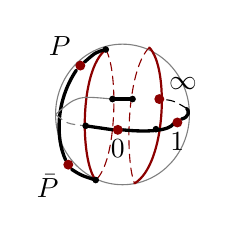
\begin{tikzpicture}[x=.85cm,y=.85cm,line cap=round,line join=round]
\draw[gray] (0,0) ellipse (1 and 1.05);
\draw[red!55!black,thick] (-.25,.97)..controls(-.65,.65)and(-.63,-.7)..(-.4,-.98);
\draw[red!55!black,densely dashed] (-.25,.97)..controls(-.06,.65)and(-.08,-.7)..(-.4,-.98);
\draw[red!55!black,densely dashed] (.4,1)..controls(.05,.65)and(.04,-.7)..(.18,-1.03);
\draw[red!55!black,thick] (.4,1)..controls(.7,.7)and(.65,-.75)..(.18,-1.03);
\draw[very thick] (-.25,.97)..controls(-.4,.93)..(-.57,.78);
\draw[very thick] (-.69,.66)..controls(-1,.2)and(-1,-.36)..(-.85,-.68);
\draw[very thick] (-.76,-.82)..controls(-.62,-.91)..(-.4,-.98);
\draw[gray,densely dashed] (-1,0)..controls(-.83,-.14)..(-.55,-.17);
\draw[very thick] (-.55,-.17)--(-.14,-.23);
\draw[very thick] (0,-.23)..controls(.4,-.27)and(.7,-.24)..(.76,-.14);
\draw[very thick] (.88,-.07)..controls(1,-.04)and(1,.05)..(.96,.09);
\draw[densely dashed] (.96,.09)..controls(.76,.21)..(.55,.23);
\draw[very thick] (-.15,.23)--(.15,.23);
\draw[gray] (-1,0)..controls(-.68,.28)..(-.15,.23);
\fill[red!55!black] (-.63,.73) circle(1.8pt) node[above left,black] {$P$};
\fill[red!55!black] (-.81,-.75) circle(1.8pt) node[below left,black] {$\bar P$};
\fill[red!55!black] (-.07,-.23) circle(1.8pt) node[below,black] {$0$};
\fill[red!55!black] (.82,-.12) circle(1.8pt) node[below,black] {$1$};
\fill[red!55!black] (.55,.23) circle(1.8pt) node[above right,black] {$\infty$};
\fill[black] (-.25,.97) circle(1.2pt);
\fill[black] (-.4,-.98) circle(1.2pt);
\fill[black] (-.55,-.17) circle(1.2pt);
\fill[black] (-.15,.23) circle(1.2pt);
\fill[black] (.15,.23) circle(1.2pt);
\fill[black] (.5,-.22) circle(1.2pt);
\end{tikzpicture}}}\\
\text{2+4 sommets-repère}\\
\text{120 structures épinglées}\\
G=1,\widetilde G=\{1,\sigma\}\end{gathered} \arrow[u,"{1\quad\gamma_r^1\quad2}"] \arrow[ur,"{3\qquad3}","{(r\in\mathrm{Rep}(K))}"',"{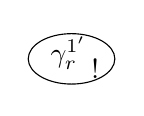
\begin{tikzpicture}[baseline=-.6ex]\draw (0,0) ellipse (.55 and .32);\node at (-.04,.07) {$\gamma_r^{1'}$};\node at (.3,-.13) {$!$};\end{tikzpicture}}"{description}] \arrow[r,"{1\quad\tau'_r\quad2}"] \& \begin{gathered}\mathrm{III}'_2\ (\text{triple triangle gauche})\\
\vcenter{\hbox{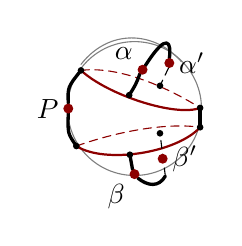
\begin{tikzpicture}[x=.85cm,y=.85cm,line cap=round,line join=round]
\draw[gray] (0,0) circle(1);
\draw[gray] (-.8,.66)..controls(-.38,1.2)and(.3,1.16)..(.7,.7);
\draw[very thick] (-.8,.57)..controls(-1,.32)..(-.99,.08);
\draw[very thick] (-.99,-.07)..controls(-1,-.37)..(-.87,-.56);
\draw[very thick] (.98,.01)--(.98,-.28);
\draw[red!55!black,thick] (-.8,.57)..controls(-.4,.2)and(.62,-.13)..(.98,.01);
\draw[red!55!black,densely dashed] (-.8,.57)..controls(-.15,.65)and(.65,.22)..(.98,.01);
\draw[red!55!black,thick] (-.87,-.56)..controls(-.45,-.83)and(.62,-.67)..(.98,-.28);
\draw[red!55!black,densely dashed] (-.87,-.56)..controls(-.1,-.29)and(.58,-.22)..(.98,-.28);
\draw[very thick] (-.08,.2)..controls(.02,.36)..(.08,.52);
\draw[very thick] (.16,.64)..controls(.5,1.17)and(.55,.98)..(.52,.75);
\draw[densely dashed] (.51,.61)--(.38,.34);
\draw[very thick] (-.07,-.69)--(-.03,-.91);
\draw[very thick] (.05,-1.04)..controls(.2,-1.16)and(.36,-1.18)..(.46,-1.01);
\draw[densely dashed] (.46,-1.01)--(.38,-.37);
\fill[red!55!black] (-.99,0) circle(1.8pt) node[left,black] {$P$};
\fill[red!55!black] (.12,.58) circle(1.8pt) node[above left,black] {$\alpha$};
\fill[red!55!black] (.52,.68) circle(1.8pt) node[right,black] {$\unsure{\alpha'}$};
\fill[red!55!black] (0,-.98) circle(1.8pt) node[below left,black] {$\unsure{\beta}$};
\fill[red!55!black] (.42,-.75) circle(1.8pt) node[right,black] {$\unsure{\beta'}$};
\fill[black] (-.8,.57) circle(1.2pt);
\fill[black] (-.08,.2) circle(1.2pt);
\fill[black] (.38,.34) circle(1.2pt);
\fill[black] (.98,.01) circle(1.2pt);
\fill[black] (-.87,-.56) circle(1.2pt);
\fill[black] (-.07,-.69) circle(1.2pt);
\fill[black] (.38,-.37) circle(1.2pt);
\fill[black] (.98,-.28) circle(1.2pt);
\end{tikzpicture}}}\quad\simeq\quad\vcenter{\hbox{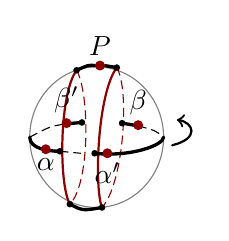
\begin{tikzpicture}[x=.85cm,y=.85cm,line cap=round,line join=round]
\draw[gray] (0,0) ellipse (1 and 1.05);
\draw[red!55!black,thick] (-.3,1)..controls(-.56,.65)and(-.57,-.7)..(-.4,-1);
\draw[red!55!black,densely dashed] (-.3,1)..controls(-.1,.65)and(-.1,-.7)..(-.4,-1);
\draw[red!55!black,thick] (.3,1.04)..controls(.01,.65)and(-.04,-.75)..(.08,-1.05);
\draw[red!55!black,densely dashed] (.3,1.04)..controls(.5,.7)and(.4,-.7)..(.08,-1.05);
\draw[very thick] (-.3,1)..controls(-.12,1.08)..(-.02,1.07);
\draw[very thick] (.12,1.07)--(.3,1.04);
\draw[very thick] (-.4,-1)..controls(-.21,-1.1)..(.08,-1.05);
\draw[very thick] (-1,0)..controls(-1,-.17)and(-.73,-.21)..(-.55,-.21);
\draw[densely dashed] (-.55,-.21)--(-.24,-.24);
\draw[very thick] (-.03,-.24)..controls(.5,-.3)and(1,-.12)..(1,0);
\draw[densely dashed] (-1,0)..controls(-.7,.16)..(-.46,.2);
\draw[very thick] (-.46,.2)--(-.22,.22);
\draw[very thick] (.38,.21)--(.62,.17);
\draw[densely dashed] (.62,.17)..controls(.88,.1)..(1,0);
\fill[red!55!black] (.05,1.07) circle(1.8pt) node[above,black] {$P$};
\fill[red!55!black] (-.76,-.18) circle(1.8pt) node[below,black] {$\alpha$};
\fill[red!55!black] (.16,-.24) circle(1.8pt) node[below,black] {$\alpha'$};
\fill[red!55!black] (-.45,.21) circle(1.8pt) node[above,black] {$\beta'$};
\fill[red!55!black] (.62,.18) circle(1.8pt) node[above,black] {$\beta$};
\draw[->,thick] (1.13,-.12)..controls(1.54,-.02)and(1.45,.22)..(1.2,.26);
\fill[black] (-.3,1) circle(1.2pt);
\fill[black] (.3,1.04) circle(1.2pt);
\fill[black] (-.4,-1) circle(1.2pt);
\fill[black] (.08,-1.05) circle(1.2pt);
\fill[black] (-.55,-.21) circle(1.2pt);
\fill[black] (-.22,.22) circle(1.2pt);
\fill[black] (-.03,-.24) circle(1.2pt);
\fill[black] (.38,.21) circle(1.2pt);
\end{tikzpicture}}}\\
\text{4+4 sommets-repère}\\
\text{60 structures de carré orienté à}\\
\text{codiagonales, }K=\{P\}\amalg I,\\
I\ \text{muni d’une \inserted{str.} carré en codiagonales }\delta=\{\{\alpha,\beta\},\{\alpha',\beta'\}\}\\
\text{i.e. d’un repère de }\unsure{\mathfrak X|\mathbb J}\unsure{(}I)\\
G=\mathbb Z/2\mathbb Z\unsure{\deleted{*}},\quad\widetilde G\simeq\mathbb Z/2\mathbb Z\times\mathbb Z/2\mathbb Z\simeq\mathbb Z/2\mathbb Z\times\{1,\sigma\}\end{gathered} \arrow[uu,bend right=70,"{1\quad\gamma_r^{2'}\quad2}"] \arrow[ull,bend left=65,"{2\quad\gamma_r^2\quad2}"']
\end{tikzcd}}
% crop-candidate: scan 31

\diagram{\[\begin{array}{lll}
\uline{\text{niveau }2}&\mathrm I_{10},\mathrm I_6,\mathrm I_4&12+20+30=62\\
\uline{\text{niveau }}1&\mathrm{II}_2,\mathrm{II}'_2,\mathrm{II}_1&60+60+120=240\\
\uline{\text{niveau }}0&\mathrm{III}_2,\mathrm{III}_{\unsure{1|4}},\mathrm{III}'_2&60+120+60=240\\
&&\overline{542}
\end{array}\]}

(l’``indice'' indique l’ordre de \(G=\operatorname{Aut}^{+}\)\unsure{;|,} donc le nb de structures est \(120/i\))

\uline{NB} Sauf \(\mathrm I_4\), toutes ces structures sont ``réelles''.

\[\begin{array}{ll}
\pi\in\mathrm{Pent}(K),&B\in\mathrm{Bit\acute et}(K)\\
s\in K,&\vec Q\in\overrightarrow{\mathrm{Carr}}(K)\\
\rho\in\mathrm{Rep}(\pi);&r\in\mathrm{Rep}(K)
\end{array}\]
(\uline{NB} \(\{(\pi,\rho)\}\unsure{\simeq}\mathrm{Rep}(K)\)).
\margin{30}
